\begin{fact}\label{iso-tri}
	Considérons tous les triangles de périmètre fixé $p$. Parmi tous ces triangles, celui d'aire maximale est le triangle équilatéral de côté $c = \dfrac13 p$.
\end{fact}


\begin{proof}
	Une première idée, calculatoire, est de passer via la classique formule de Héron $Aire = \sqrt{s(s - a)(s - b)(s - c)}$ où $s = \num{.5} p$ désigne le demi-périmètre, et les variables $a$, $b$ et $c$ les mesures des côtés du triangle. Concrètement, comme l'aire est positive ou nulle, il suffit de chercher les minimums de $Aire^2 = s(s - a)(s - b)(s - c)$. Ceci fonctionne, mais n'est pas accessible à un collégien, ni même à un lycéen qui ne sait pas différentier une fonction de plusieurs variables.%
	\footnote{
		XXXX
		
		L'ensemble des valeurs possibles de $a$, $b$ et $c$ est un compact, quitte à accepter des triangles dégénérés, donc  atteint son minimum.
		Comme de plus, les antécédents de ce minimum doivent annuler $\pder{A_s}{a}{1}$, $\pder{A_s}{b}{1}$ et $\pder{A_s}{c}{1}$, et $A_s(a;b;c)$ est une fonction symétrique en $a$, $b$ et $c$, nous savons que le minimum est atteint en $(\frac13 p ; \frac13 p ; \frac13 p)$. 
	}
	Il se trouve que l'on peut établir l'affirmation \ref{iso-tri} ci-dessus avec des raisonnements géométriques élémentaires.
	La petite astuce toute simple est de considérer le problème plus contraint exprimé dans le fait \ref{iso-tri-one-side-fixed} ci-dessous qui permet de conclure comme suit.
	%
	\begin{itemize}
		\item 

		\item 

		\item 
	\end{itemize}
\end{proof}


% ----------------------- %


\begin{fact}\label{iso-tri-one-side-fixed}
	Considérons tous les triangles de périmètre fixé $p$ et ayant tous au moins un côté de même mesure $c$. Parmi tous ces triangles, celui qui a une aire maximale est le triangle isocèle ayant une base de mesure $c$.
\end{fact}


\begin{proof}
	XXXX

	\begin{center}
		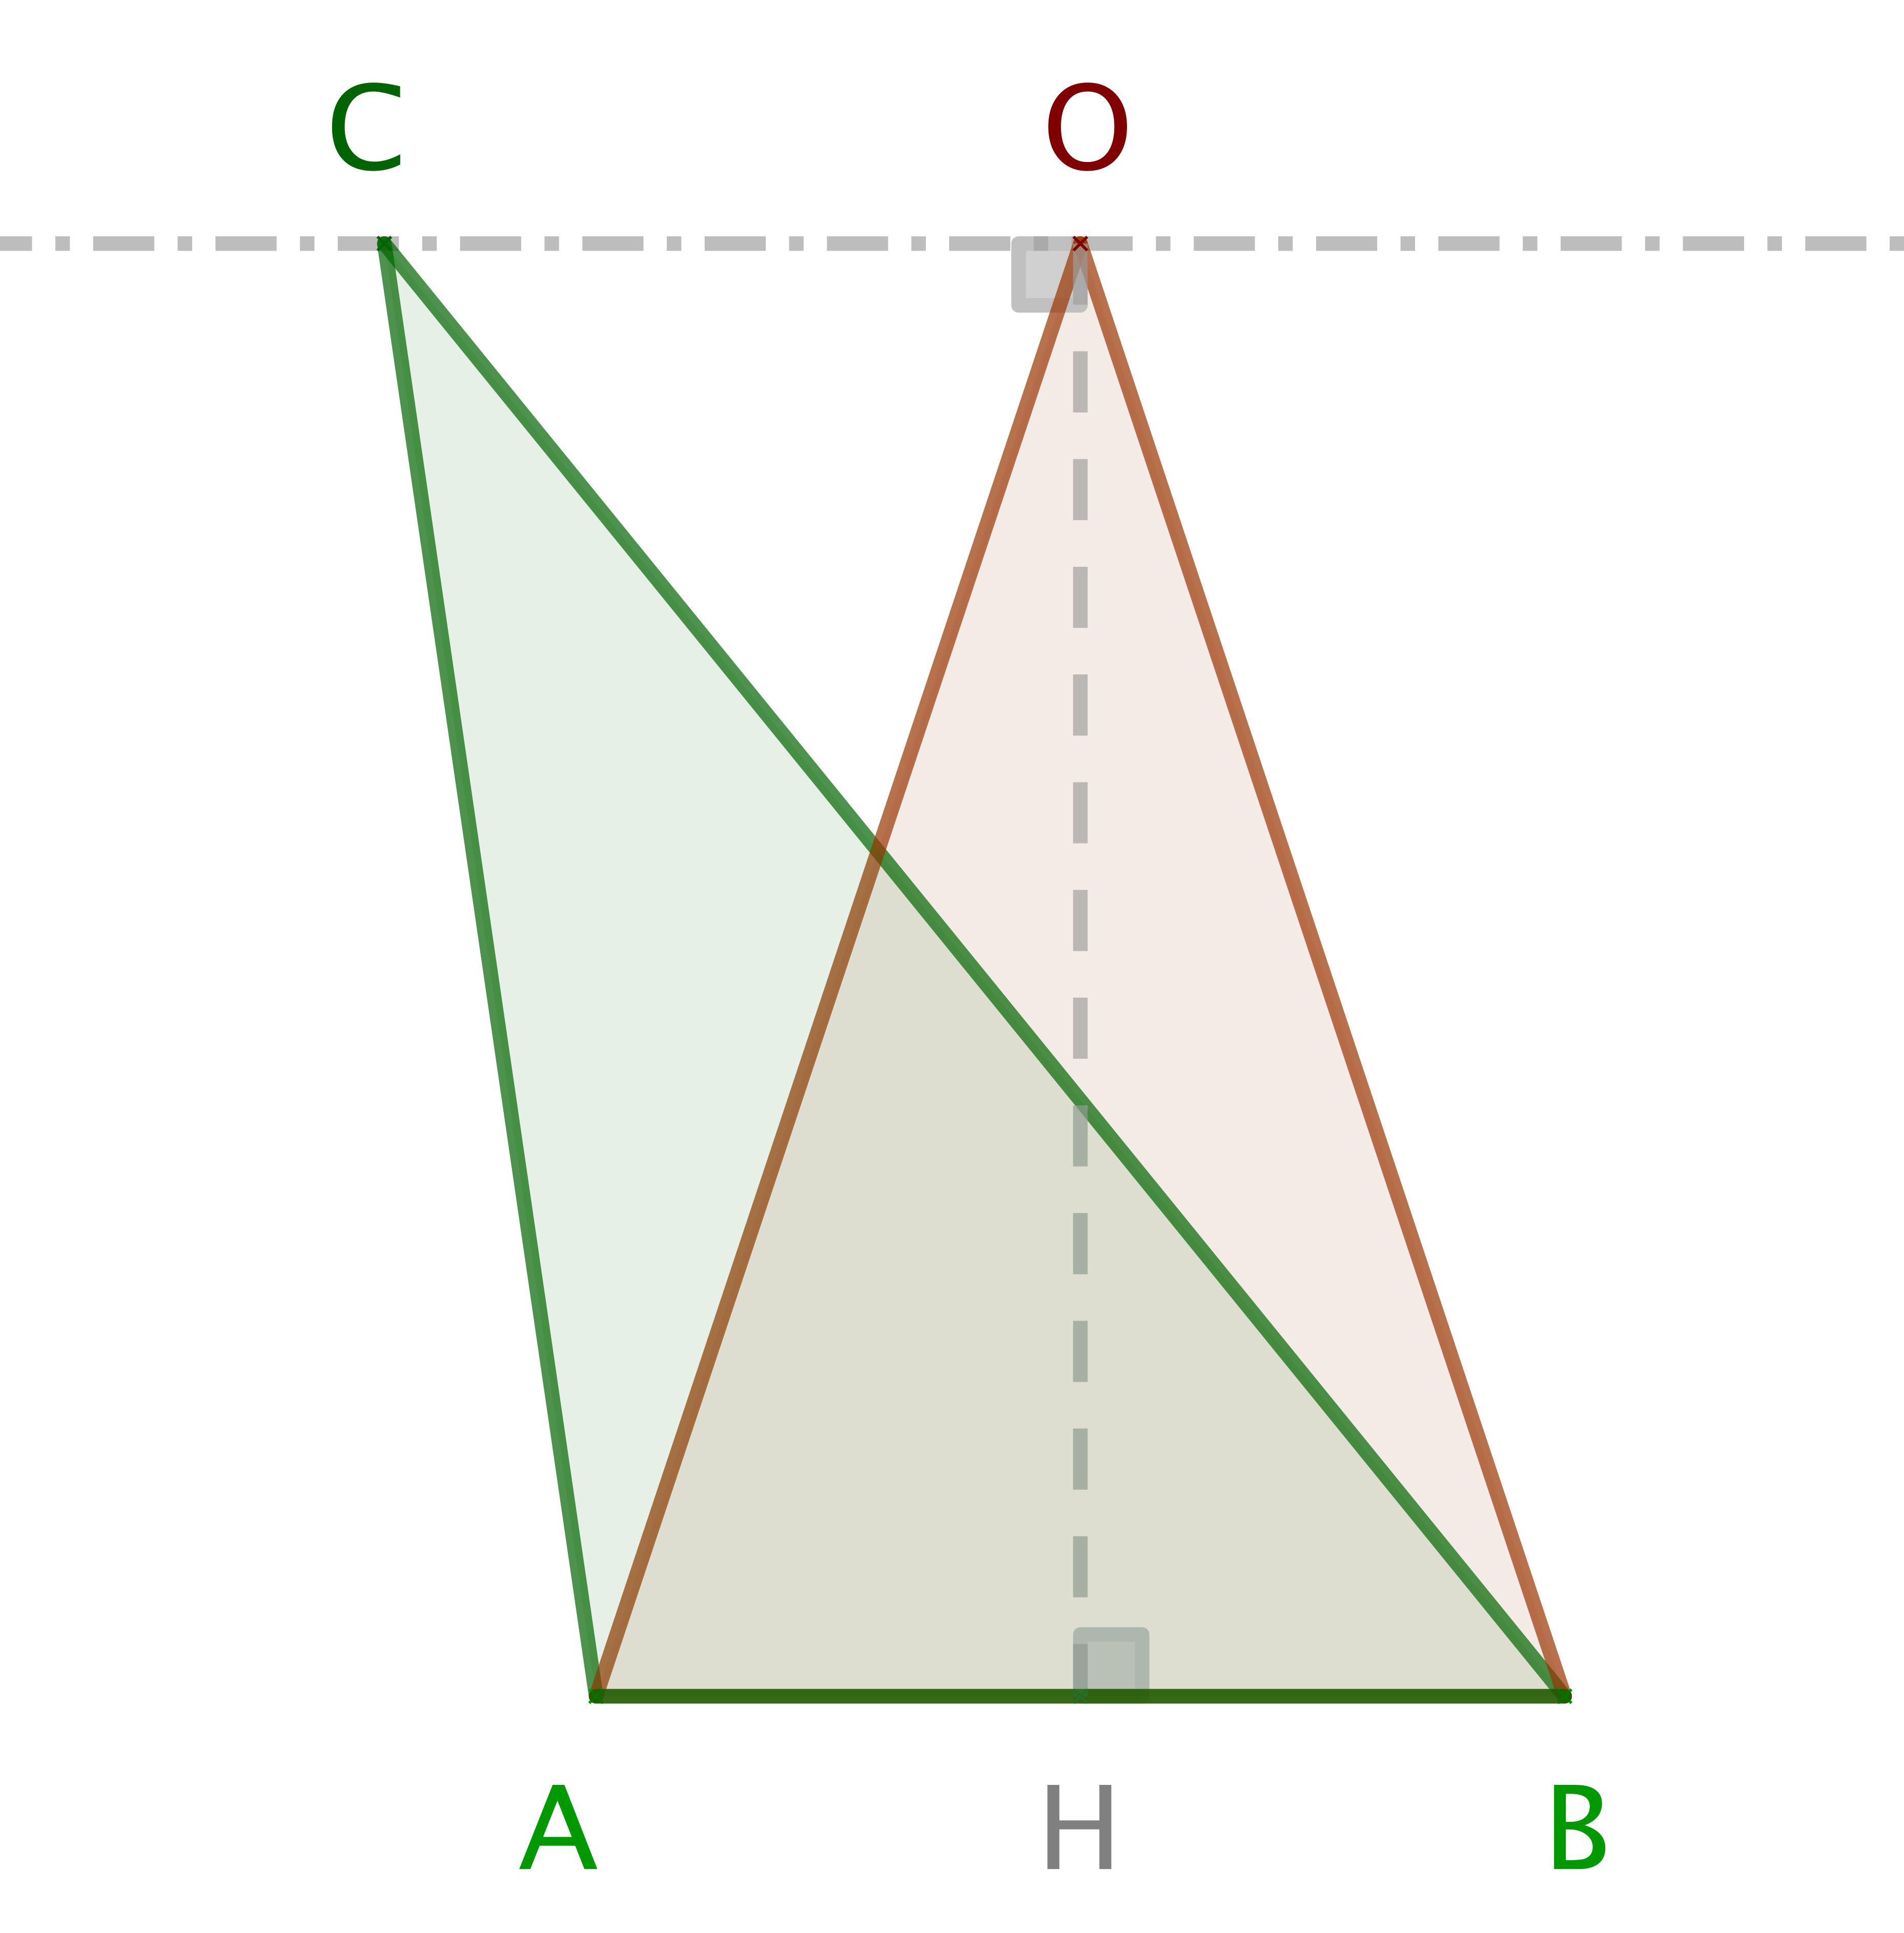
\includegraphics[scale=.4]{content/triangle/triangle.png}
	\end{center}

	\begin{center}
		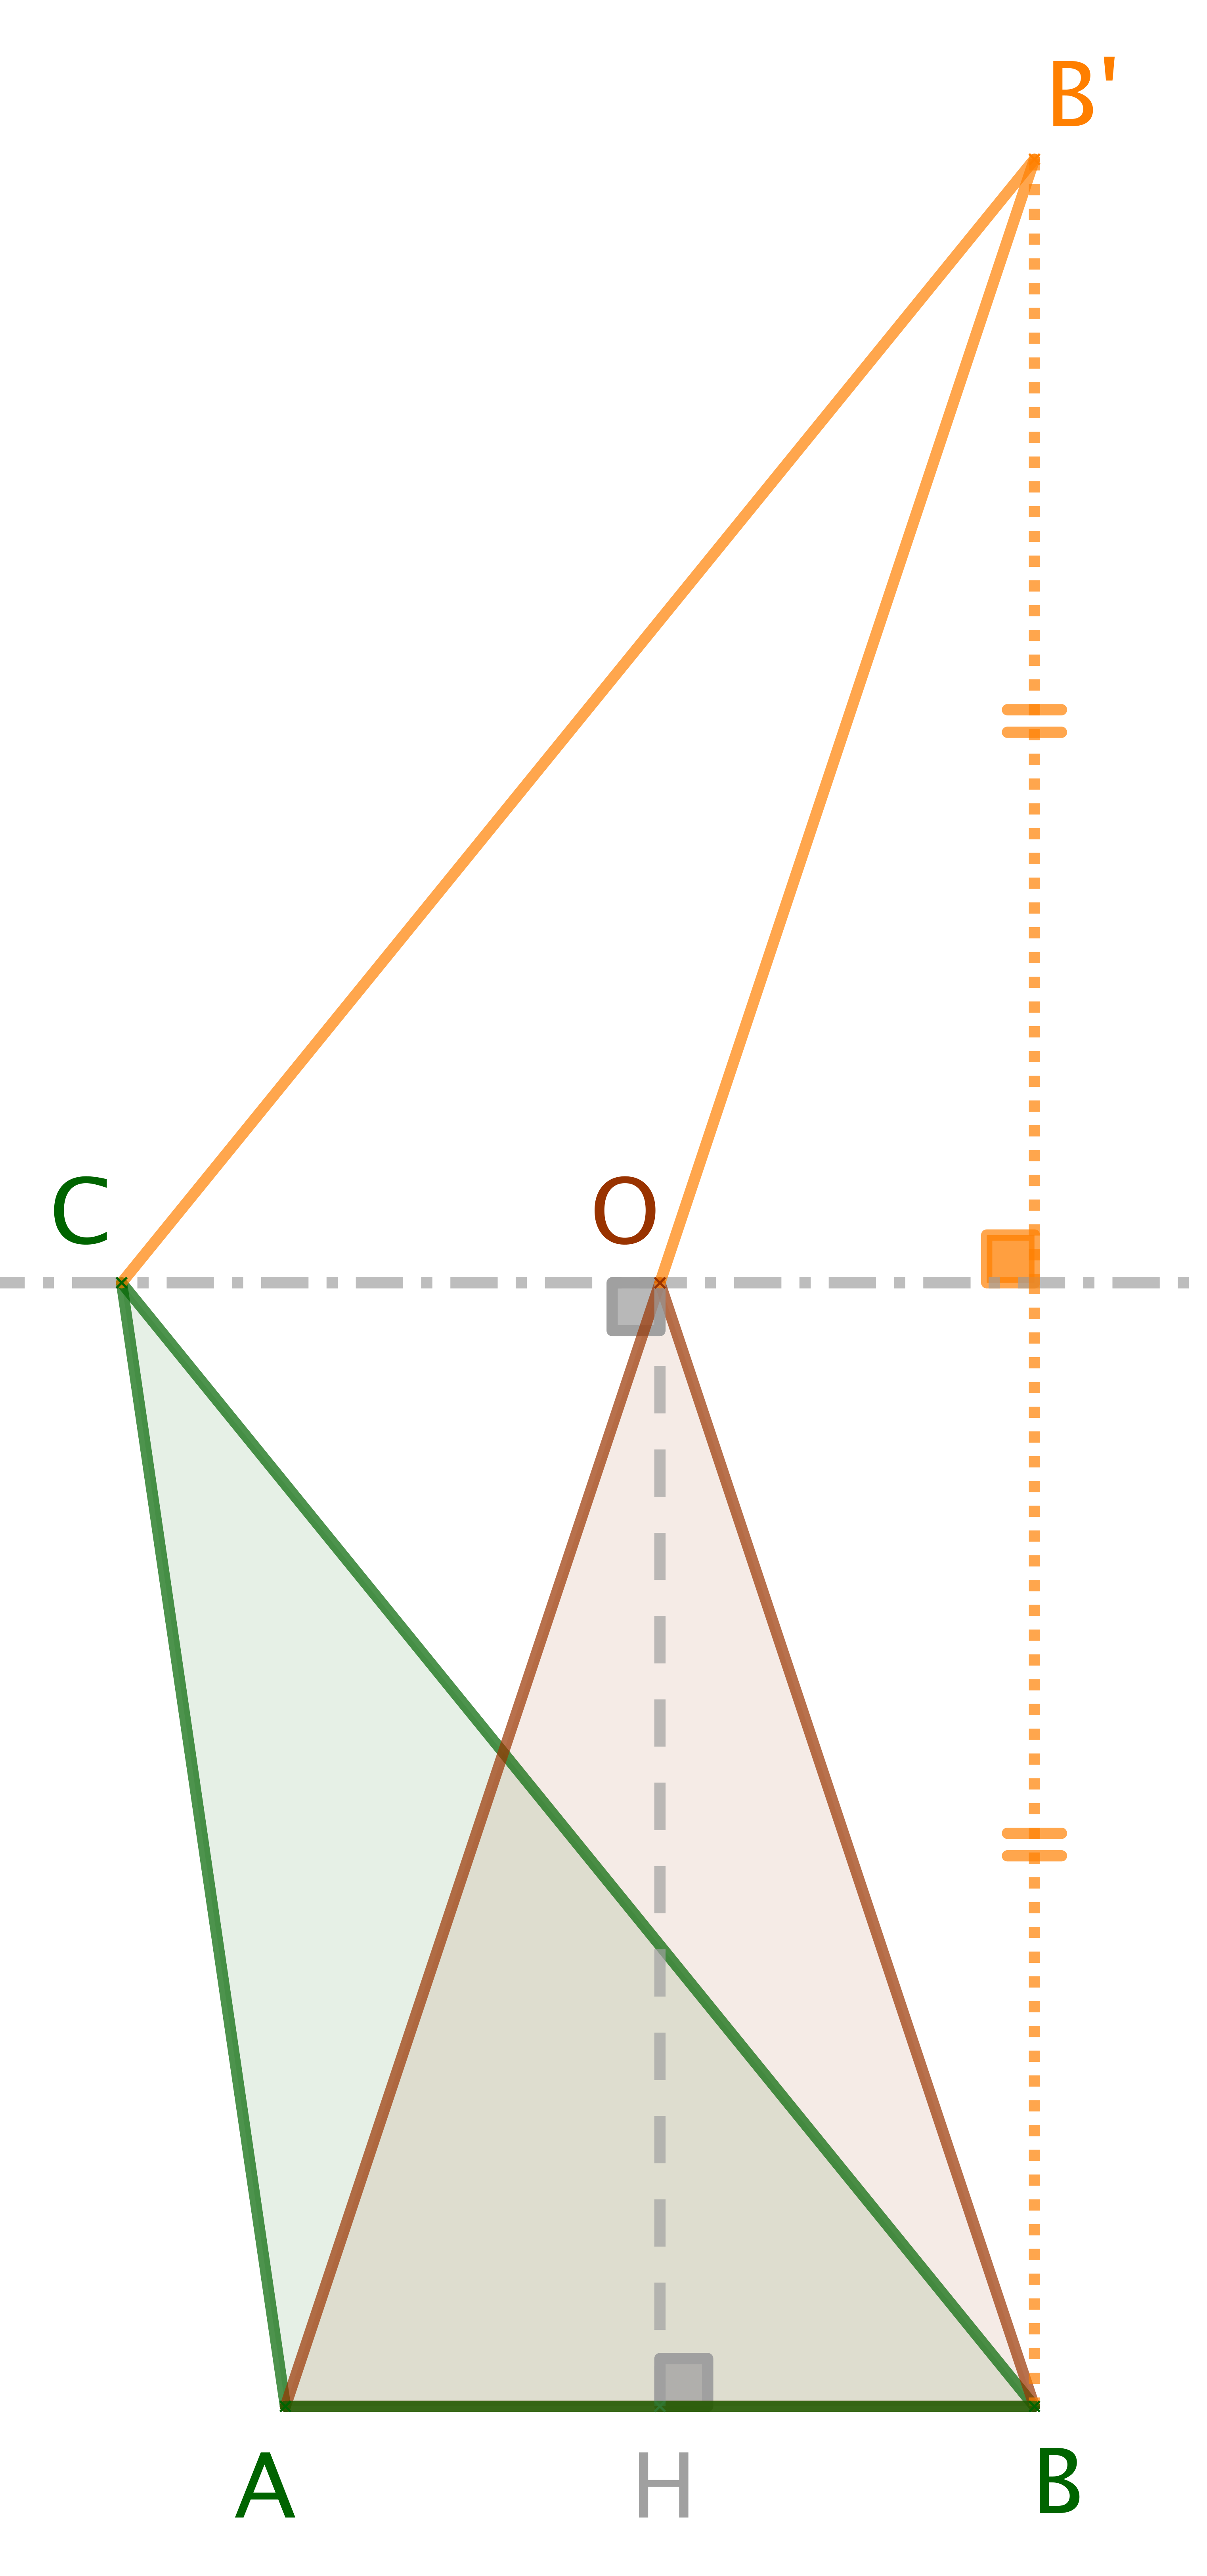
\includegraphics[scale=.4]{content/triangle/triangle-proof.png}
	\end{center}
	
	YYYY
	
	
	Joli! Non?
\end{proof}